\documentclass[10pt]{report}
\usepackage{graphicx}
\usepackage{a4}
\usepackage{url}

% Report template authored V. Sorge, adapted S. Vickers.

\title{% This is the title of your document
  {\normalsize Software Workshop Team Java (06-08165) 2010/11, Dr E. Thompson }\\[2cm]
  Project Report:\\
  An Applet to Demonstrate ...}
\author{Team A2:  \\
  Jeremiah Via \\
  Joss Greenway \\
  Yukun Wang \\
  Charlie Horell
}

\begin{document}

\maketitle
\chapter*{Work Breakdown}
\label{work-breakdown}

\thispagestyle{empty}


{\small
  \noindent\begin{tabular}{|l||l|l|l|l|l|}\hline
    \textbf{Coding} & \textbf{Dino (Team Leader)} & \textbf{Fred} & \textbf{Wilma} & \textbf{Barney} & \textbf{Betty} \\ \hline\hline
    Datastructures  & Contribution: 100\%         & 0\%           & 0\%            & 0\%             & 0\%            \\ \hline
    \ldots          & \ldots                      & \ldots        & \ldots         & \ldots          & \ldots         \\ \hline
  \end{tabular}\vspace*{1cm}

  \noindent\begin{tabular}{|l||l|l|l|l|l|}\hline
    \textbf{Report} & \textbf{Dino (Team Leader)}           & \textbf{Fred} & \textbf{Wilma} & \textbf{Barney} & \textbf{Betty} \\ \hline\hline
    Introduction    & Chapter~\ref{cha:introduction}: 100\% & 0\%           & 0\%            & 0\%             & 0\%            \\ \hline
    \ldots          & \ldots                                & \ldots        & \ldots         & \ldots          & \ldots         \\ \hline
  \end{tabular}
}

\tableofcontents
\thispagestyle{empty}

\begin{abstract}
  You should write a one-page abstract written as an ``Executive Summary''. It
  should be written for someone who is familiar with the Team Java module, so
  that there is no need for background or generalities. Rather, you should
  explain what is special about your project, and what you claim to have
  achieved. (One page maximum.)
\end{abstract}


\chapter{Introduction}
\label{cha:introduction}

% Give a brief overview and guide the reader to the important points
% in the following sections.  Tell your reader what you are going to
% tell them. Overview the project highlighting the issues you
% addressed and hinting at how you solved them. The reader should be
% able to decide from the introduction what parts of the report are of
% interest to them

This report aims to document how our team was able to create a
game. We had roughly 10 weeks to create a game from start to
finish. This was a new experience for all of us and we learned many
lessons from it. We are all better programmers now and we have a
better idea of what it means to create software with a team.

We will begin by describing the final specification of our game. It
changed from our initial specification as we learned more about game
programming. This was a new domain for all of us so our initial ideas
of what it meant to make a game morphed as we gained experience in the
field. We will also explain why we chose the features we did and how
those features positively affect the user experience.

After going over the specification, we will go into the design of our
game. This section will go into the vital details of our game
architecture. You will learn about problems we encountered when
implementing features and how we solved them. We want to not only tell
you what architectural choices we made but why we made them. This will
give you insight into our problem solving abilities as a team.

We will then tell you about how we tested our game and validated its
user experience. This is an important section and we aim to highlight
how extreme programming methodologies allowed us to create good
software. We will show you how unit testing allowed us to assert our
intended uses of the code and ensure future feature enhancements would
be prevented from breaking old, stable code.

With testing and validation out of the way, we will talk about how we
managed our project. Because this was our first experience writing
code as a team, it presented us with new opportunities for
learning. We will discuss how extreme programming helped us maintain
forward momentum on our game and how utilising pair programming
ensured that everyone understood the code to a sufficient level.

We would like to wrap our report up with a general discussion of how
the module was for us. Programming a game from start to finish as a
team was a novel experience. As a result of this we made mistakes. We
will talk about the mistakes we made as a team and individually and
the lessons we learned from them. Because of this module we have an
increased maturity in our programming, meaning that we can recognise
the long-term issues with the choices we make.


\section{Initial Ideas}


At our first meeting we considered various games and discussed many
ideas. We debated the merits of various games and ended up deciding on
criterion for a good game. The game we would make would need to lend
itself to an iterative release schedule. This was important so that we
could add new features each week. We wanted to avoid anything that
would require multiple weeks to implement. We also wanted a game that
would be fun to play. This was a challenge because many entertaining
games have a lot of complex features. These two criterion constrained
our search for a game to make.


Ideas for games that were ultimately rejected included:

\begin{description}
\item [Fruit Ninja] A game which involved the slicing of fruit with a
  blade controlled by the mouse. This game was rejected because we
  could add nothing original to it or come up with any particularly
  fun or innovating multiplayer modes other than a who can post the
  highest score style game.

\item [Tower Defence] A game involving the placing of towers and
  weapons to destroy enemies that work their way through a level. This
  could possibly be made multiplayer in a cooperative mode.

\item [Zombie Tower Defence] As above but involving zombies. We
  rejected both the tower defence games as we felt they had been done
  many times before and lacked originality. There were also free
  versions available of the game online that were very playable.

\item [Space Racing Game] A racing game which takes place in space
  where the players must race while avoiding planets and
  asteroids. This was rejected again for lack of originality.
\end{description}


The game we finally settled on was a multiplayer version of Osmos
developed by Hemisphere games \cite{osmos}. We called our game
Darkmatter as we would be setting it in space with the concept of
stars rather than on the cellular level like Osmos.

All of us were happy with this selection as it included features that
played to the strengths of all members of the team. Joss with the
potential to produce exciting graphics and audio effects, Charlie with
the chance to use his physics knowledge and Jeremiah and Yukun to
utilise their strong programming skills.

%%% Local Variables: 
%%% mode: latex
%%% TeX-master: "../report"
%%% End: 

%  LocalWords:  Osmos Darkmatter Joss morphed multiplayer Yukun


\chapter{Requirements}
\label{cha:requirements}

You have been given only a very general set of requirements; hence
you have to formulate more specific and detailed user requirements
for the applet you chose to do and explain why you chose these
features. Explain your choices carefully (not just lists of bullet
points). Note that not everything about requirements in general is
relevant for this project (for instance, you need not write much
about the hardware requirements, as they are trivial for this
project).


\chapter{Design}
\label{cha:design}

This section is crucial. Describe the overall structure of your
program at a suitably high level of abstraction. For instance, UML
diagrams or informal box-and-arrow diagrams can be used to describe
program structure. Be sure to describe the MVC structure used. Note
that code listings or screenshots are not appropriate here. An
important point is how you have divided the project into modules
that different team members can work on, and how these are then
integrated. For example, you could use interfaces to describe a
clean boundary between modules, so that some team members use the
functionality provided by the interface, while another team member
implements it. Bear in mind Software Engineering principles of good
design like coherence and coupling.

\chapter{Validation and Testing}
\label{cha:validation}

% Establish what your project can handle successfully, and what its
% limitations are. Use meaningful examples, not lists of trivial
% cases.
%
% Your applet is expected to be in good working order and do something
% useful. This chapter is important, because it describes how you
% assure yourself that that is the case.
% 
% Establish what your project can handle successfully, and what its
% limitations are. Use meaningful examples, not lists of trivial
% cases.

Testing and validation are important aspects of extreme programming
and we did our best to remain faithful to the traditional
approach. Our testing strategy never became very complicated; there
was not enough time to develop a more comprehensive approach. Had
there been time, we would have liked to add integration tests to our
project.

\section{Testing}

Because our team adopted the extreme programming methodoloy, testing
was an important part of our development process. Our pair programming
sessions usually consisted of three stages, the second one being the
creation of unit tests for the code we just wrote. We took advantage
of JUnit in order to create a series of consitent tests. Our aim was
to have as much test coverage as possible. It was not about simply
creating a test for each method but instead ceating a test for each
behavior we intended the method to have. It is for this reason that we
have multiple tests for some methods.

Our testing strategy was quite simple. We created test suites at the
package level and tested all the behaviour we wanted our code to be
able to deal with. This meant identifying potential weak spots in the
code and testing for it. Our process fell short of the test-driven
approach of writing tests first but we still did a good job of
creating tests to make our code fail. We envisioned every way in which
our code could potentially fail and wrote a test for it. This meant
having a lot of failling code at first but as we refined our methods
and assumptions we gradually passed more tests until we passed them
all.

Testing the whole of our project was done in a visual and interactive
way. Part of this was because we did not create integration tests to
test the behaviour of multiple subsystems working
together. Integration tests were outside the scope of our assignment
but we still regret not exploring and implementing them. The other
reason we had to test our game interactively was simply due to the
domain in which we were programming. Games present a challenge for
automated testing. While it would be possible to test some behaviour
with Java's GUI robots, it is a lot harder to put a test into numbers
when we are aiming to test the \emph{feeling} of the game. For these
kinds of tests we simply had to play the game a lot. This was not a
problem, though, as we all enjoyed playing our game. The added benefit
of play-testing the game was that it would excite us to add or enhance
game features.

% Testing is so you can be confident that the software is robust and
% bug-free. What was your strategy for that? How did you plan unit
% testing (for components) and integration testing (for the whole
% applet)? How did the prototype fit in?

% Ideas: 
%
% - We never tested what happens if more players connect to the server
% than there are matter objects on the map.
%

\section{Validation}

Validation was a very informal process for our team. Since we were the
kinds of users our game was intended for, we were able to determine if
the software was headed in the right direction. Because of our weekly
release process, we could review the current state of the game at each
meeting. By each meeting we had coded our respective parts and were
now all together, we could voice opinions on the way the software
worked. This was done multiple times throughout the development of our
game.

Weekly validation was critical to make the zooming and scrooling
features of the game work well. When discussing the feature and how it
worked, we undoubtedly envisioned subtlely different variations as to
how it would look. After a prototype was created we all talked about
it. This input allowed a refinement of the behaviour that we all felt
worked well.

A similar situation happened with the absorption of matter objects. It
took many iterations to get the absroption behaviour exactly
correct. There were many details to consider, such as absorption rate
and change in momentum, whch made working out the exact behaviour we
wanted take a long time. Each week we were able to see a slightly
modified absorption behaviour and by voicing our opinions it reached
its final, excellent state.

% Validation is to check that in the end the applet is useful
% and pleasant to use. What was your strategy for that? Have you tried
% it out with teachers or students? What kind of rolling validation
% did you use for the evolutionary part (developing the GUI)?



%%% Local Variables: 
%%% mode: latex
%%% TeX-master: "../report"
%%% End: 

\chapter{Project Management}
\label{cha:management}

% The week-to-week management of your project is documented in your
% weekly progress reports, so you do not need to repeat that
% information here. A number of important points that you need to
% address are: how you divided up the work, allocated team members to
% particular tasks, coordinated what team members were working on, and
% communicated the relevant technical information in the team.
%
% Note that a clean design makes all of these easier, so you could
% refer to your design section where appropriate.
%
% You should also discuss difficulties in the team interactions if
% there were any, and how you dealt with them. This section is vital
% for the assessment of your team work and engineering practices.
%
% - Software engineering practices that have been used on
% the project are described including the identification
% of how they were adapted to the projects
% requirements.
%
% - The practices have been evaluated with respect to the
% effectiveness in relation to the project and alternative
% ways for approaching the project have been identified
% and described.
%
% - The report tries to be realistic about the practices and not
% simply trying to be idealistic or paint a good picture


At our first meeting we discussed the required roles needed for a
successful team. We decided that our team needed a \emph{Team Leader}
to guide the project and make executive decisions when
required. Additionally we decided we needed a \emph{Team Secretary} to
keep the administration work up-to-date and to organise meetings and
liaise with demonstrators and module coordinators. All members of the
team were also designated as \emph{Software Developers} to emphasise
that we were all there to write code together. Our team structure
was: \begin{inparaenum}[\itshape a\upshape)]
\item Joss Greenaway as Team Leader,
\item Charles Horrell as Team Seceretary,
\item Yukun Wang as Software Developer and
\item Jeremiah Via as Software Deveoper
\end{inparaenum}.

We decided to have one meeting a week in addition to our meeting with
our demonstrator, Katrina Samperi. This was deemed necessary to keep
the team in constant contact and decide on weekly and long-term
goals. We made ourselves a Facebook group to maintain contact between
the team.

Minutes of all meetings were uploaded to Subversion to keep the team
abreast of weekly goals. Weekly reports were produced containing our
weekly goals as well as a review of the past week. These were
extremely useful in assessing and evaluating our own performance over
the previous week and scheduling work for the week ahead.

\begin{wrapfigure}{r}{8cm}
  \begin{tabular}{|r|c|c|c|c|} \hline
    & Tuesday      & Thursday                   \\ \hline
    10:00 & Team Meeting &                      \\ \hline
    11:00 & Sessions One &                      \\ \hline
    12:00 &              & Session Two          \\ \hline
    13:00 &              &                      \\ \hline
    14:00 &              & Session Three        \\ \hline
    15:00 &              & Demonstrator Meeting \\ \hline
  \end{tabular}
  \caption{Weekly Meetings}
  \label{fig:schedule}
\end{wrapfigure}

We also scheduled pair programming sessions three times a week as
shown in Figure \ref{fig:schedule}. This was one of our favourite
aspects of the agile methodology. Because of pair programming
sessions, we were all aware of design decisions and how they impacted
code. We were also able to find bugs quickly and create better
software overall. Our pair programming sessions allowed each of us to
program with everyone on the team. This was great because it gave us
the chance to work with others of differing abilities and to be
exposed to different ways of problem solving. Our three sessions were
organized as follows:

\begin{enumerate}
\item
  Joss and Jeremiah \\
  Charlie and Yukun
\item
  Charlie and Jeremiah \\
  Joss and Yukun
\item
  Joss and Charlie \\
  Yukun and Jeremiah
\end{enumerate}

The Tuesday morning meeting was mainly used for deciding on goals for
the week ahead and reflection.  There were many features which we
wanted to get into the game. It is during this time that we would
decide which features were the most critical. By defining the critical
goals we were one step closer to actually getting a working game. We
would also use this time to reflect on our performance over the past
week and discuss any issues that had arisen in the code. Additionally,
we used this time to give feedback on other's code and suggest
possible improvements or altenatives. Charlie would take minutes of
our meetings which would then be available for reference throughout
the week. This was useful for ensuring that we were all working
towards the game goal.

It was useful having a pair programming session immediately after our
meeting. The meeting would get us excited to add new features to our
game. It was often after a meeting that a state of ``feature clairty''
would posses us and cause us to become extremely productive. During
these sessions we traditionally wrote a class file, as many tests to
make it fail as we could think of, revisions to make the class pass
those tests and then the documentation necessary. This pattern caused
to implement the bulk of our code and make sure that everyone worked
together to make it.

Our meeting with Katrina was used for evaluation and feedback from the
previous week. These were meetings where we would show Katrina the
current state of our game and solicit feedback from her. She would
also give us ideas on how to plan and when to begin woking on aspects
of our project. Having her guidance was immensely helpful because it
functioned as a verification of our process. During one week in
particular, we all fell behind in our game due to other
deadlines. Katrina was quick to remind us that we have a finite amount
of time to finish this game and that we must always be spending a set
amount of time on it. With her input we were able to maintain an
overall forward momentum on our game and anticipate problems that
would arise in our software.

\section{Subversion}

We used Subversion a lot and considered it a tremendous asset to our
development process. Our repository was organised the traditional way
with three folders for the \texttt{trunk}, \texttt{tags} and
\texttt{branches} of our code. We never actually made use of the
\texttt{branches} directory due to one team member's bad experience
merging different branches of code. Our goal was to create a tagged
release of our code each week but we fell bhind considerably on this
goal. It was hard to remember to tag a branch instead of continuing in
the development process.

We all had different styles of using Subversion. Some committed to the
repository every time they had a small but functioning block of code
whereas others would wait until they had a more substantial amount of
code to commit. Fortunately, this was not hard to work around. All of
our IDEs had built-in tools to resolve the conflicts that arose so our
differnt styles never created a real impedence to our development.

Subversion can become complicated when all the team members begin
committing their IDE specific files and the output of the buld
process. Fortunately, we were able to use Subversion's
\texttt{svn:ignore} property to prevent these kinds of files from
being added. The basic criteria for adding a file to the ignore pattern
was if it was automatcally generated from a tool. This ensured our
directories were clean and prevented the sorts of conflicts caused by
build files.

Subversion was used to host all of our documentation as well. This
meant that meeting minutes, schedules, mock-ups and other miscellany
we kept in one conveninent location as reference for the whole team.

In order to make our lives easier, we imposed some of the rules on our
repository suggested at the beginning of the module. First, we made it
a rule that no code could be submiteed to the repository which failed
any unit tests. Lastly, all code commits needed a message explaining
\emph{why} these changes had been made. Combined, these two rules
ensured that we had no trouble using Subversion over the course of our
project.

\section{Maven}

Another critical component of our build process was Apache
Maven. Maven is a build tool for Java which works at a higher level
than Ant \cite{maven} . It also imposed a set of best practices on the
development process which aided in our development. By doing things
the Maven way, we were able to get a lot for free.

For example, a Maven project is created with JUnit as a
depenedency. This means that any of us can immediately begin working
with the code and run unit tests. We never had to worry about
downloading the right version of JUnit and adding it to our project
manually. Maven installs all dependencies to a local repository on
each of our machines. This means that we can keep \texttt{jar}s out of
the repository which saves space. In fact, through our whole
development process we never had a \texttt{jar} archive in our
repository. There was simply no need because at any time we could run
\texttt{mvn package} and one would be generate for us after passing
all of our unit tests.

Rather than deal with the incompatible build files for a number of
different IDEs, we were able to simply run the Maven project
as-is. All IDEs have the ability to work with Maven projects, either
built-in or through an official plug-in. This meant that we could
develop according to the Maven life-cycle in any IDE. This
freed us from fighting with IDE-specific build files and meant that we
could all have our own settings.

Maven can generate site documentation and Java documentation as
well. This was very useful. We always had a version of our site and
Java documentation hosted on the internet. Because of this we always
had useful information about our project. Maven's site documentation
includes useful components like a page to check the code style against
that of Sun's Java Guidelines. It would also give statistics on the
unit tests such as coverage and how many were passing.

Overall, Maven made our lives a whole lot easier and we heartily
recommend teaching it next year the same way JUnit was taught this
year.


\section{Software Engineering Approach and Principles}

We decided that our main software engineering approach would be
\emph{extreme programming} which is one of the agile programming
methodologies. This methodology focuses on using many short release
cycles. These cycles include producing a small feature set during each
iteration, producing the relevant unit tests and documenting it for
our own future reference. It also places an emphasis on pair
programming and other strongly cohesive team activities.

The benefits of this methodology to us were numerous. For example, the
short release cycles favoured by extreme programming were convenient
for us because we only had nine weeks to produce the project. This
gave us nine iterations in which to plan features and distribute the
work required for the game. It also favoured our approach of weekly
meetings and progress reports. This meant that for the Thursday
meetings with our demonstrator, we had a new iteration of working code
to show. It also suited Subversion because we could have a lot of
smaller commits.

By breaking the project up into these weekly cycles it also allowed us
to spread the work as evenly over the term as possible. This was
better than having to rush to finish and test the game at the end. By
constantly testing our game and using unit tests throughout our
development, we could be sure that the code we produced was working as
we expected. This was better for our small team than using a non-agile
method such as the Cleanroom method which only would have slowed us
down. This is because we would not be able to guarantee until the
final stages of testing that our game will worked how we wanted. Our
agile methodology meant that our project was low risk.

Another advantage was the fact that extreme programming builds from
the bottom up. We were able to quickly get a simple prototype of the
game working early on in its simplest form. Each week we could add
features and polish to the game. This fitted in with our schedule and
short deadlines as it ensured that we built on the game, week on week,
rather than trying to develop some extremely complicated features that
would in the end not be implemented. It meant that if we did not meet
all our aims and implement all the desired features our game would
still be working to a high enough standard.

We also liked the integrated teamwork associated with extreme
programming. Our team wholeheartedly took up the practise of pair
programming. We met for sessions at least three times a week as
detailed in \ref{fig:schedule} above. These were useful to the team as
it allowed everyone in the team to contribute code and work with every
other member of the team. This ensured that everyone kept in touch
with one another and was aware of all aspects of the project. It also
allowed for our stronger coders to help our weaker ones. It gave
everyone a chance to work on each section of the code and created
bug-catching redundancy because there were more eyes on the code. With
the exception of networking, no single person was assigned an entire
task to complete on their own so there was always someone else ready
to help with coding or solving a problem.

Testing was an important part of our software engineering philosophy,
we aimed to cover as much of our functionality with unit tests as we
could. We made it a criteria that everyone submit unit tests with the
code they created. For this reason, we had one unit test for every 80
lines of code (including comments). We feel confident in our code
because were able to ensure our code worked consistently for all edge
cases we could think of.

\subsection{Other Methodologies}

We considered other software engineering methodologies early on in the
development cycle. After some research and debate, we settled on
extreme programming. Here were our evaluations of other techniques
which we decided not to use.

Initially we had considered Scrum \cite{sutherland2004} but decided it
was not appropriate for our circumstances. We did not have a product
owner which made using the technique difficult (although it would have
been possible to use Katrina for this role). Also, our team was a
smaller size than the traditional Scrum team and we wanted to have a
shorter release cycle. A key reason this approach would not work for
us was the daily meeting. Since we all had other modules we could not
work out a way to meet everyday. These reasons caused us to abandon
Scrum as a contender for our development process.

We also discarded Waterfall because of the uncertainty involved and
the need for a long design phase at the start which went against our
natural desire to start coding as soon as possible. There was also the
danger of not being able to test our code until the end of the project
and the fears that it would not work. We were also advised against
this methodology by many guest lecturers for the course. We were also
not entirely certain at the start of the project what we needed to do.
Because we had to do some exploratory programming, the Waterfall
approach of big design up front would have been ill-suited to
us. Having to stick to our initial conceptions of what the project
should be like would be extremely constricting whereas an agile
development process would allow us more freedom and flexibility.

\section{Release Plan}

We adopted a modified extreme programming cycle; we would have a new
release each week. At the beginning of each week, we would have a few
features that we wanted to add. That entire week would be spent on
coding them and making them robust and well documented. At the
beginning of the next week, we would review what we did well and
poorly over the last week and see how we can improve our
processes. Our release cycle worked like the one shown in Figure
\ref{fig:gantt}.

\begin{figure}
  \begin{gantt}{12}{10}
    \begin{ganttitle}
      \numtitle{1}{1}{10}{1}
    \end{ganttitle}
    \ganttbar{Physics}{0}{1}
    \ganttbarcon{Animation}{1}{1}
    \ganttbarcon{Game Prototype}{2}{1}
    \ganttbarcon{Scrolling}{3}{4}
    \ganttbarcon{Menu}{7}{3}
    \ganttbar{Level Loader}{4}{2}
    \ganttbarcon{Level Editor}{9}{1}
    \ganttbar{Networking}{5}{3}
    \ganttbar{Music}{8}{1}
    \ganttbar{Human Player}{3}{1}
    \ganttbarcon{AI Player}{4}{6}
  \end{gantt}
  \caption{A Retrospective Project Schedule}
  \label{fig:gantt}
\end{figure}

This approach allowed us to have a working and playable game at every
stage of development. By gradually adding features on top a
well-tested and documented core, we could be more productive. Less
time needed to be spent fixing broken code. Our aim was to have a
stable, minimal working product every week. We also wanted to create a
tag each week with what we accomplished and use this as a frame of
reference to see how our code is progressing. Unfortunately, we did
not quite live up to that desire.

% Our Release Plan was decided upon in-line with extreme methodology. We
% intended to update to a new release for every team Java week that is
% for every Tuesday we would move onto a new release. This was in-line
% with extreme methodology as it placed an emphasis on short small
% working releases every week.

% \begin{wrapfigure}{r}{7cm}
%   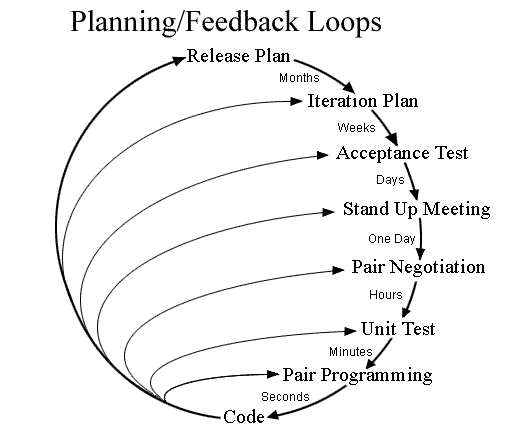
\includegraphics[width=0.5\textwidth,keepaspectratio]{img/xp-cycle.png}
%   \caption{Diagram of the XP work cycle}
% \end{wrapfigure}

% We followed this diagram for the most part apart from our release plan
% took place over a much shorter cycle as we effectively only had 9
% weeks to produce our entire project. This was a significant advantage
% over other software engineering philosophies as it allowed us to adapt
% our goals to produce work over a short time at a consistent pace and
% under considerably less uncertainty and pressure than following
% something like waterfall.


% \begin{wrapfigure}{r}{8cm}
  % \begin{tabular}{l p{12cm}}
  %   Week  & Goals \\ \hline
  %   1     & Meet with team, contact demonstrator, organise first meetings. Decide on Game. \\
  %   2     & Produce initial sandbox designs and decide on team structure and roles. \\
  %   3     & Have working basic game.\\
  %   4     & Improve basic game, add backgrounds and music.\\
  %   5     & Add AI player, start networking.\\
  %   6     & Add extra levels, Implement scrolling.\\
  %   7     & Working networking.\\
  %   8     & Menu, credits.\\
  %   9     & Sprite Graphics and Weapons features.\\
  %   10    & Polishing off game, Final report, Demonstrate Game.\\
  %   11    & Finish final report and hand in. \\
  % \end{tabular}
  % \caption{Our idealised development schedule}
  % \label{fig:ideal-schedule}
% \end{wrapfigure}



%% LocalWords:  Samperi Horrell Greenway Joss Facebook Yukun XP organise api

%%% Local Variables:
%%% mode: latex
%%% TeX-master: "../report"
%%% End:
% LocalWords:  emphasise favourite organised IDEs IDE intellij netbeans SCRUM
% LocalWords:  Scrum keepaspectratio img workpackages gant timeplan Workpackage
% LocalWords:  eps JUnit depenedency internet Cleanroom


\chapter{Conclusions}
\label{chap:conclusions}


Evaluate what you have achieved in your project in objective terms
(not just things like ``we are all happy with the result''). What
are the strenths and limitations of your project? If you had more
time, what could you add? If you could do it all over again, what
would you do differently? Are there general things about software or
team management that you have learnt in this project that you could
apply if you were going to work on a (perhaps completely different)
team project in the future?


\bibliographystyle{plain}
\bibliography{report}

Acknowledge any code you have used (if any), and also any that was
generated automatically, e.g. by wizards.

Give correct and complete bibliographic information for any sources
cited. See the local referencing guide. For instance cite which
books on software engineering you have used, for
instance~\cite{software-design}. Use the \texttt{report.bib} file to
manage your citations.

When you \emph{quote} material from other sources, you must be
absolutely clear \emph{at the point where you quote it} exactly
which of your material is quoted and what the source is. As
explained in \cite{SoCS:plagiarism},

``Direct quotation is not particularly common in scientific writing,
as it is generally not the words that matter, but the meaning.
Normally it is preferable to rewrite someone else's ideas in your
own words, often changing the terminology and other superficial
details to suit the new context.

However, in circumstances where it is appropriate to make direct use
of the words of another person, those words should normally be
included within quotation marks and a reference to the source of the
words given in the usual way.''

\end{document}
